\section{Software empleado en el proyecto}
\subsection{ROS}
ROS (Robotic Operating System) consite en un framework para la robótica sobre el que desarrolladores de cualquier 
ambito pueden aportar soluciones modulares a los sistemas de forma general. La modularidad de ROS hace que desarrollar 
un nuevo sistema o prototipo pueda ser una tarea tan sencilla como interconectar módulos de otros desarrolladores con 
los propios.
\begin{comment}
Esta característica lo hace idoneo para un proyecto como este en el que el uso de técnicas de percepción, 
mapeado, localization, etc, complejas se escapa del alcance; y solo sea necesario el desarrollo de modulos específicos de este robot
que sean capaces de comunicarse con aquellos más complejos y sean capaces de proporcionarle los datos necesarios para implementar los
algoritmos de SLAM. \\    
\end{comment}


El sistema operativo empleado tanto en el ordenador de abordo del robot,la Raspberry Pi, cómo en en el ordenador principal es Ubuntu 16.04, de tal modo que la distro de ROS en la que ha sido 
implementado el proyecto es ROS Kinetic Kame\footnote{https://wiki.ros.org/kinetic}.
\begin{figure}[!ht]
    \centering
    
\includegraphics[width=0.3\textwidth]{images/kinetic.png}
    \caption{Version de ROS empleada}
\end{figure}

\subsubsection{Interfaz con IMU}
Como ya se ha visto en la seccion \ref{imu_hardw}, al robot se le ha dotado con una IMU de seis grados de libertad con el fin de obtener medidas de aceleraciones.\\
La conexión se hace a través de una linea por protocolo $I^2C$, por lo que ha sido necesario el desarrollo de dos `wrapers' en Python con funciones de bajo nivel; uno para el acceso a las
funciones de comunicación $I^2C$ a nivel de registros hardware y otro a nivel de funcionalidades elementales para el manejo de los datos de la IMU.
Sobre ambos `wrapers' se ha escrito el nodo de ROS encargado de publicar los datos en dos `topics', \textit{imu1\_rawImu} y \textit{imu1\_scaImu}, con los datos tal y como llegan 
de la IMU en el primero y reescalados en el segundo. El tipo de mensaje en el que se publican los datos es \textit{\href{http://docs.ros.org/kinetic/api/sensor_msgs/html/msg/Imu.html}{sensor\_msgs/Imu}}.\par
Al tratarse de un sensor de bajo nivel que aporta información a los estratos más bajos del control, para poder disponer depués de mayor ancho de banda, se ha elegido una frecuencia de muestreo del sensor de $50\ [Hz]$; sufucientemente alta para no comprometer la estabildiad del sistema
pero tambien lo sufucientemente baja como para no saturar el ordenador de abordo (teniendo en cuenta que este también deberá mantener un flujo constante de imagenes capturadas por la cámara, con el coste que eso conlleva).

 \subsubsection{Interfaz con encoders}\label{enc_soft}
Otro sensor añadido son los encoders mencionados en la sección \ref{enc_hard}. Para su programación se ha desarrollado un `wraper' en C++ de la librería para Raspberr-Pi 3B \textit{pigpio} 
\cite{pigpio}. Como los encoders solo pueden ofrecer información de la magnitud de la velocidad y no del sentido de giro, es necesario realizar dicha consideración a nivel de software para poder representar esa información.
Esto se consigue suscribiéndose al `topic' \textit{cmd\_vel}, obtiniéndose así la referencia del sentido de giro a cada lado del robot. Este dato se usa para reajustar el signo de las velocidades leídas de los seis encoders y publicarlas en el topic \textit{encoders} con el tipo de mensaje \textit{\href{http://docs.ros.org/jade/api/std_msgs/html/msg/Float64MultiArray.html}{std\_msgs/Float64MultiArray}}. La medida de los encoders, al tratarse de medidas de baja calidad con valores dispersos, son filtradas y promediadas entre sí. En cuanto a la frecuencia de muestreo, se ha seguido la misma filosofia que con la programación del nodo de la IMU y se ha decido muestrear a $50\ [Hz]$.

\subsubsection{Odometría}
A partir del calculo de la velocidad obtenida desde los encoders se desarrolló un nodo en ROS en el que se calcula la odometría del robot.\\
Para ello se han hecho una serie de suposiciones y simplificaciones del modelo del robot que después, en base a los resultados obtenidos, se han demostrado bastante acertadas.
\begin{itemize}
    \item Las ruedas tienen un modelo de rodadura perfecto y no deslizan en el suelo; esto no es cierto en la práctica, y supone una fuente de errores importantes por la deriva que acumulan las posiciones estimadas. Dichos errores que son corregidos mediante una fusión sensorial.
    \item El modelo del robot consiste en un modelo diferencial de dos ruedas. En base a esto, a cada rueda `virtual' se le asigna el promedio de la velocidad de las 3 ruedas de cada bancada.
\end{itemize}
Las ecuaciones que definen el modelo del robot son las mostradas a continuación:
\begin{figure}[!ht]
    \centering
    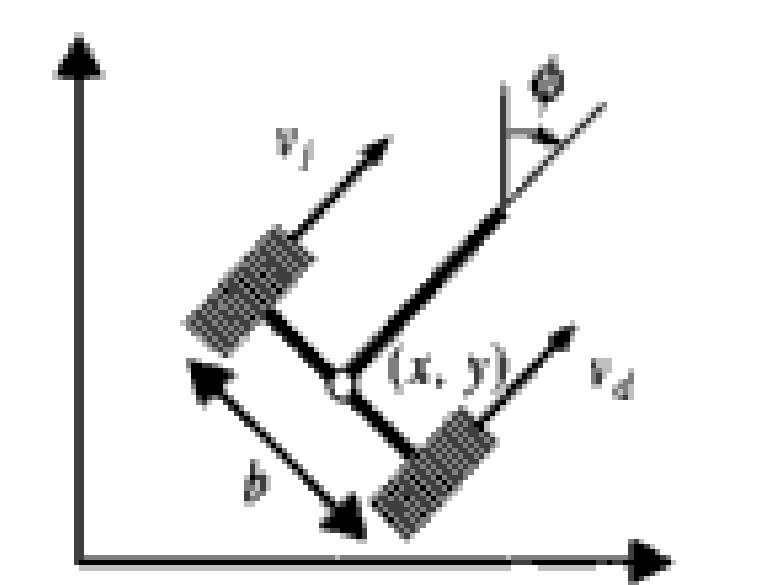
\includegraphics[width=0.3\textwidth]{images/dif_model}
    \caption{Representación posición y orientación modelo diferencial}
\end{figure}
\begin{center}
    $v=\dfrac{v_{dcha}+v_{izqd}}{2}$ \hspace{2cm} $\theta=\dfrac{v_{dcha}-v_{izqd}}{b}$
\end{center}
dónde \textit{v} es la velocidad lineal, \textit{w} la velocidad angular y \textit{b} la distancia entre las ruedas.\\
Se define la posición y la orientación del robot cómo:
\begin{equation}
    \begin{pmatrix}
        \dot{x} \\
        \dot{y} \\
        \dot{\theta}
    \end{pmatrix}=
    \begin{pmatrix}
        cos(\phi) & 0 \\
        sin(\phi) & 0 \\
        0 & 1 \\
    \end{pmatrix}
    \begin{pmatrix}
        v \\
        \theta
    \end{pmatrix}
\end{equation}
\par
Este nodo se suscribe al desarrollado en \ref{enc_soft} en el `topic' \textit{encoders}, y cada vez que llega un mensaje nuevo con los datos de los 
encoders calcula el avance del robot en base al modelo propuesto. La publicación de los datos se hace en el `topic' \textit{odom} a un ratio de $25\ [Hz]$ con un mensaje del tipo \textit{\href{http://docs.ros.org/kinetic/api/nav_msgs/html/msg/Odometry.html}{nav\_msgs/Odometry}}.

\subsubsection{Interfaz Raspberry-Pi/Arduino}
La comunicación por puerto serie se implementa haciendo uso de la librería \textit{CmdMessenger} \cite{CmdMessenger}, que permite definir comandos (con la posibilidad de asociarles argumentos y callbacks) de forma eficiente y sencilla.
Por la parte de la Raspberry, se usan las librerías CmdMessenger (desarrollada en C) o su alternativa PyCmdMessenger (en Python) en el nodo \textit{serial\_com.py} para transmitir por el puerto serie. Los siguientes comandos son los más importantes: \\
\begin{itemize}
	\item \textbf{Cmd\_off} $\rightarrow$ Al recibir este comando el micro pasa a no hacer nada, comportándose como un apagado de emergencia.
	\item \textbf{Change\_ref} $\rightarrow$ Acompañado de un valor de referencia de la velocidad, que el micro usará para el control de los motores.
\end{itemize}
\par
De este modo es sencillo publicar un tópico de 'comandos del sistema', como apagar o funciones de debugeo, y otros tópicos para los datos que hayan de retransmitirse. Cuando llegan datos desde el arduino, se ejecuta un callback (de la librería externa, no de ROS) que publica dicha información el tópico correspondiente. Si es el caso contrario, y se busca enviar datos al arduino, el nodo se subscribirá al tópico con ese dato y en el callback asociado (ahora sí de ROS) se envía al arduino.

\subsubsection{Interfaz Arduino/Motores}
Una interrupción disparada a partir de uno de los timers del microcontrolador ejecuta el control de bajo nivel, garantizando un tiempo de actuación para el controlador con una periocidad constante. Al ser un vehículo puramente diferencial, todos los motores de un mismo lado se mueven en la misma dirección. Sin embargo, debido a la gran diferencia entre las respuestas de los motores, la señal de control de cada uno debe ser única. Por tanto, las señales necesarias para controlar los motores son; dos digitales por cada lado del vehículo para configurar la dirección del mismo, y una señal analógica generada por PWM para cada motor para modificar su velocidad. \\
Una vez realizados los cálculos, y escritas las señales para controlar los motores, se procede, si da tiempo antes de la próxima ejeccución de la interrupción, a recibir referencias u órdenes desde la Raspberry Pi. El control es un simple PI cuyas ganancias han sido ajustadas experimentalmente, con un \textit{anti-windup} con constante de tiempo configurable.

\subsubsection{Computación distribuida con ROS-Multimaster Package}
Las técnicas de SLAM a testear en el robot desarrollado son computacionalmente costosas. Todo este coste computacional es
imposible asumirlo desde una Raspberry-Pi, por lo que surge la necesidad de hacer el procesado en un servidor remoto \textit{on the fly} con las 
dificultades que eso conlleva, entre ellas y la más importante, la sincronización de datos. Bajo estas condiciones de diseño y restricciones aparece una solución de la comunidad: ROS multimaster\_fkie. La premisa que lo rige es simple, dado un sistema mutirobot cada elemento mantiene la ejecución de dos nodos locales, \textit{master\_discovery} y \textit{master\_sync}; el primero es el encargado de mantener una lista del resto de \textit{roscores} disponibles en la red y de publicar el suyo propio como activo, el otro es el encargado de suscribir su \textit{core} a los nodos de otros \textit{cores}. Así, todas las unidades de procesamiento tienen acceso a los recursos del resto. 
\begin{figure}[!ht]
    \centering
    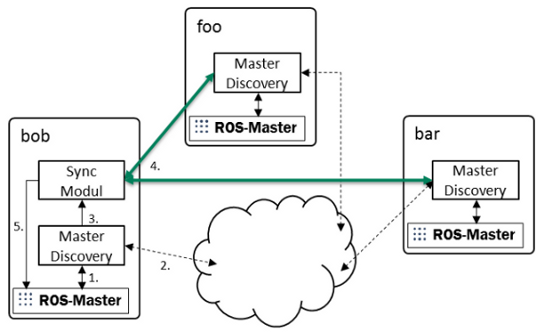
\includegraphics[width=0.6\textwidth]{images/ros_multimaster.png}
    \caption{Esquema del funcionamiento básico del paquete Multimaster}
\end{figure}

En este proyecto, su integración se ha llevado a cabo lanzando en la Raspberry-Pi y en otro PC los nodos correspondientes; siendo la Raspberry-Pi la 
suministradora de información y el PC el encargado de procesarla.

\subsection{Implementación filtro estadístico}
Debido a los múltiples sensores que integra el robot, a la variedad de sus medidas y a las incertidumbres, desconocidas, a la que están sujetos, se ha considerado necesario y tremendamente benificioso la implementación de algún tipo de \textit{Data Fusion}. Con este objetivo se introduce un filtro estadístico, de Kalman, para estimar el vector de estados del vehículo. La razón por la que se ha elegido este filtro frente a otros, por ejemplo un filtro de información, se debe a la simpleza del modelo de observación, pues las posibles entradas son meramente la odometría de los encoders, las medidas de la IMU y la odemetría visual.

\subsubsection{Filtro de Kalman Extendido}
La información que el sistema obtiene de los sensores está sujeta a ruido e incertidumbres de la medida. A fin de minimizar los errores y mejorar la estimación de la posicion y velocidad del robot se ha 
considerado que era de especial interes y utilidad la aplicación de un filtro recursivo Bayesiano como estimador de estados, en concreto el filtro de Kalman extendido. \\
Este filtro es una extensión del filtro de Kalman para sistemas no lineales.
\begin{figure}
    \centering
    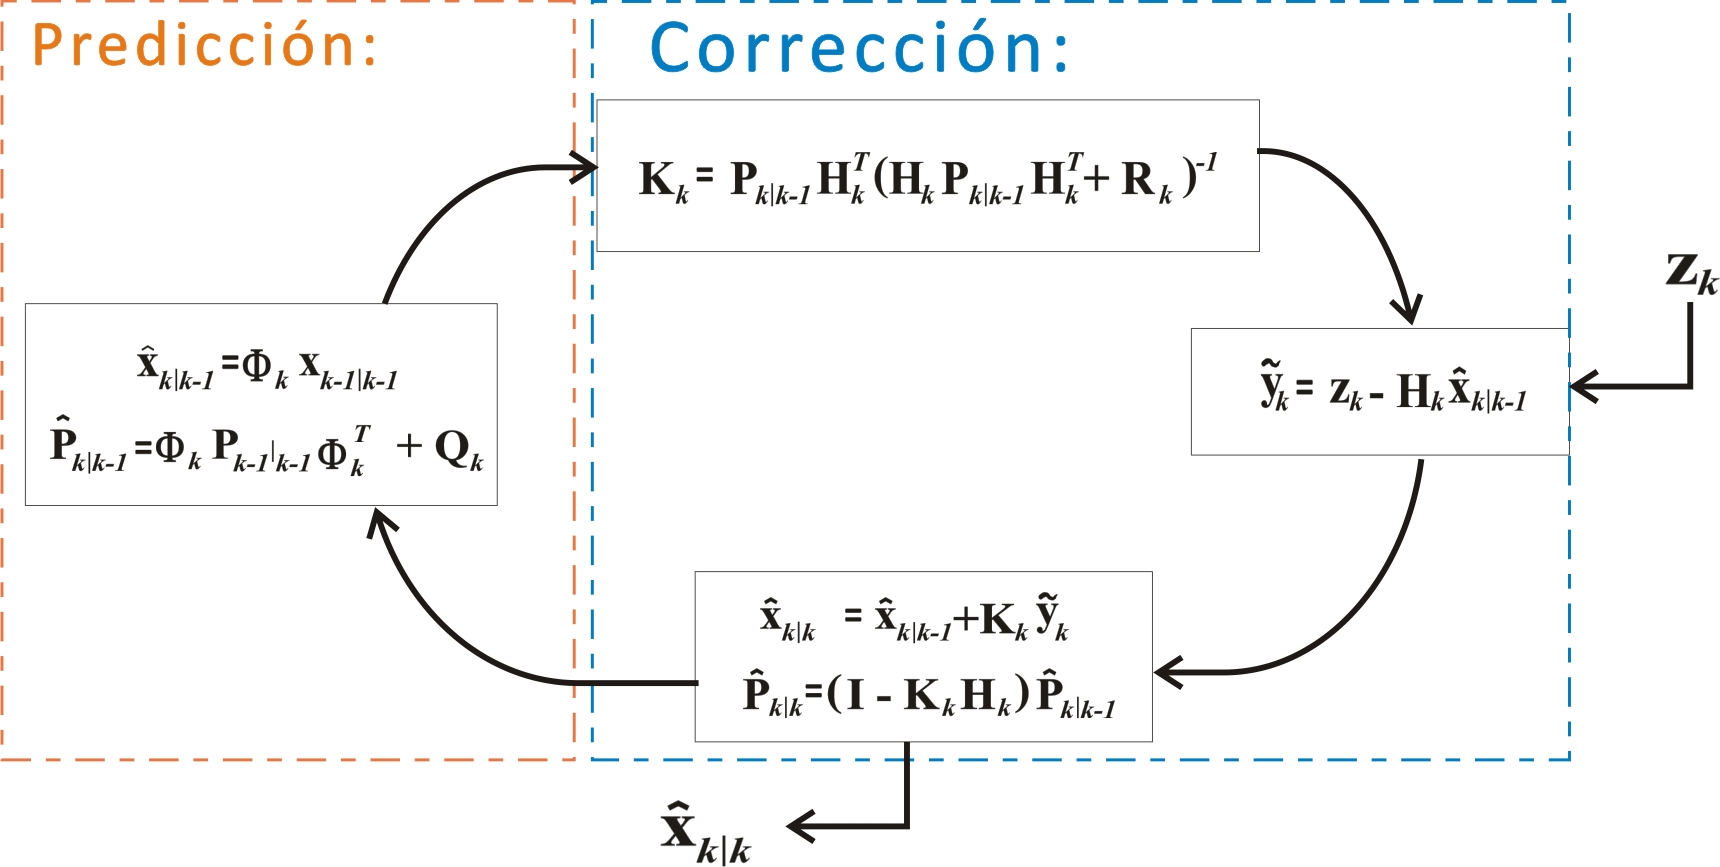
\includegraphics[width=0.8\textwidth]{images/kalman.jpg}
    \caption{Representación del filtro de Kalman. Fuente: Wikipedia}
\end{figure}

\subsubsection{ROS-Robot Localization Package}
Como implementación del EKF se ha decidido usar el paquete de ROS kinetic \textit{Robot Localization}\cite{MooreStouchKeneralizedEkf2014}. Este paquete contiene dos nodos de estimación de estados, uno con un filtro extendido y el segundo con un \textit{Unscented Kallman Filter}. Además integra utilidades que facilitan el uso de un sistema GPS, cuyos detalles serán ignorados aquí por resultar irrevelantes para este proyecto.\\
Las capacidades interesantes de este paquete las podemos resumir en las siguientes:
\begin{itemize}
	\item Múltiple entrada de sensores, sin restricción en número o tipo.
	\item Configuración sencilla de las entradas, pudiendo descartar ciertas medidas o corregir determinados datos de antemano.
	\item Tanto los sensores como el comportamiento del modelo se ajusta fácilmente desde un fichero yaml.
	\item Los nodos estiman un estado 15-dimensional del robot: posición (X,Y,Z), orientación (\textit{pitch},\textit{roll},\textit{yaw}), velocidad, tanto de la posición como de la orientacion, y aceleración del robot.
	\item Soporte de los mensajes de ROS para cada tipo de sensor y sus estándares.
\end{itemize} 

\newpage

\subsection{Arquitectura general del sistema}
A continuación, se mostrará la comunicación entre nodos tanto dentro de la RPi cómo en el momento de lanzar las técnicas de SLAM. En primer lugar se mostrará la estructura en el momento en el que se grabó
el \textit{bag} y, cómo sería la estructura si se realizará SLAM :
\begin{figure}[!ht]
    \centering
    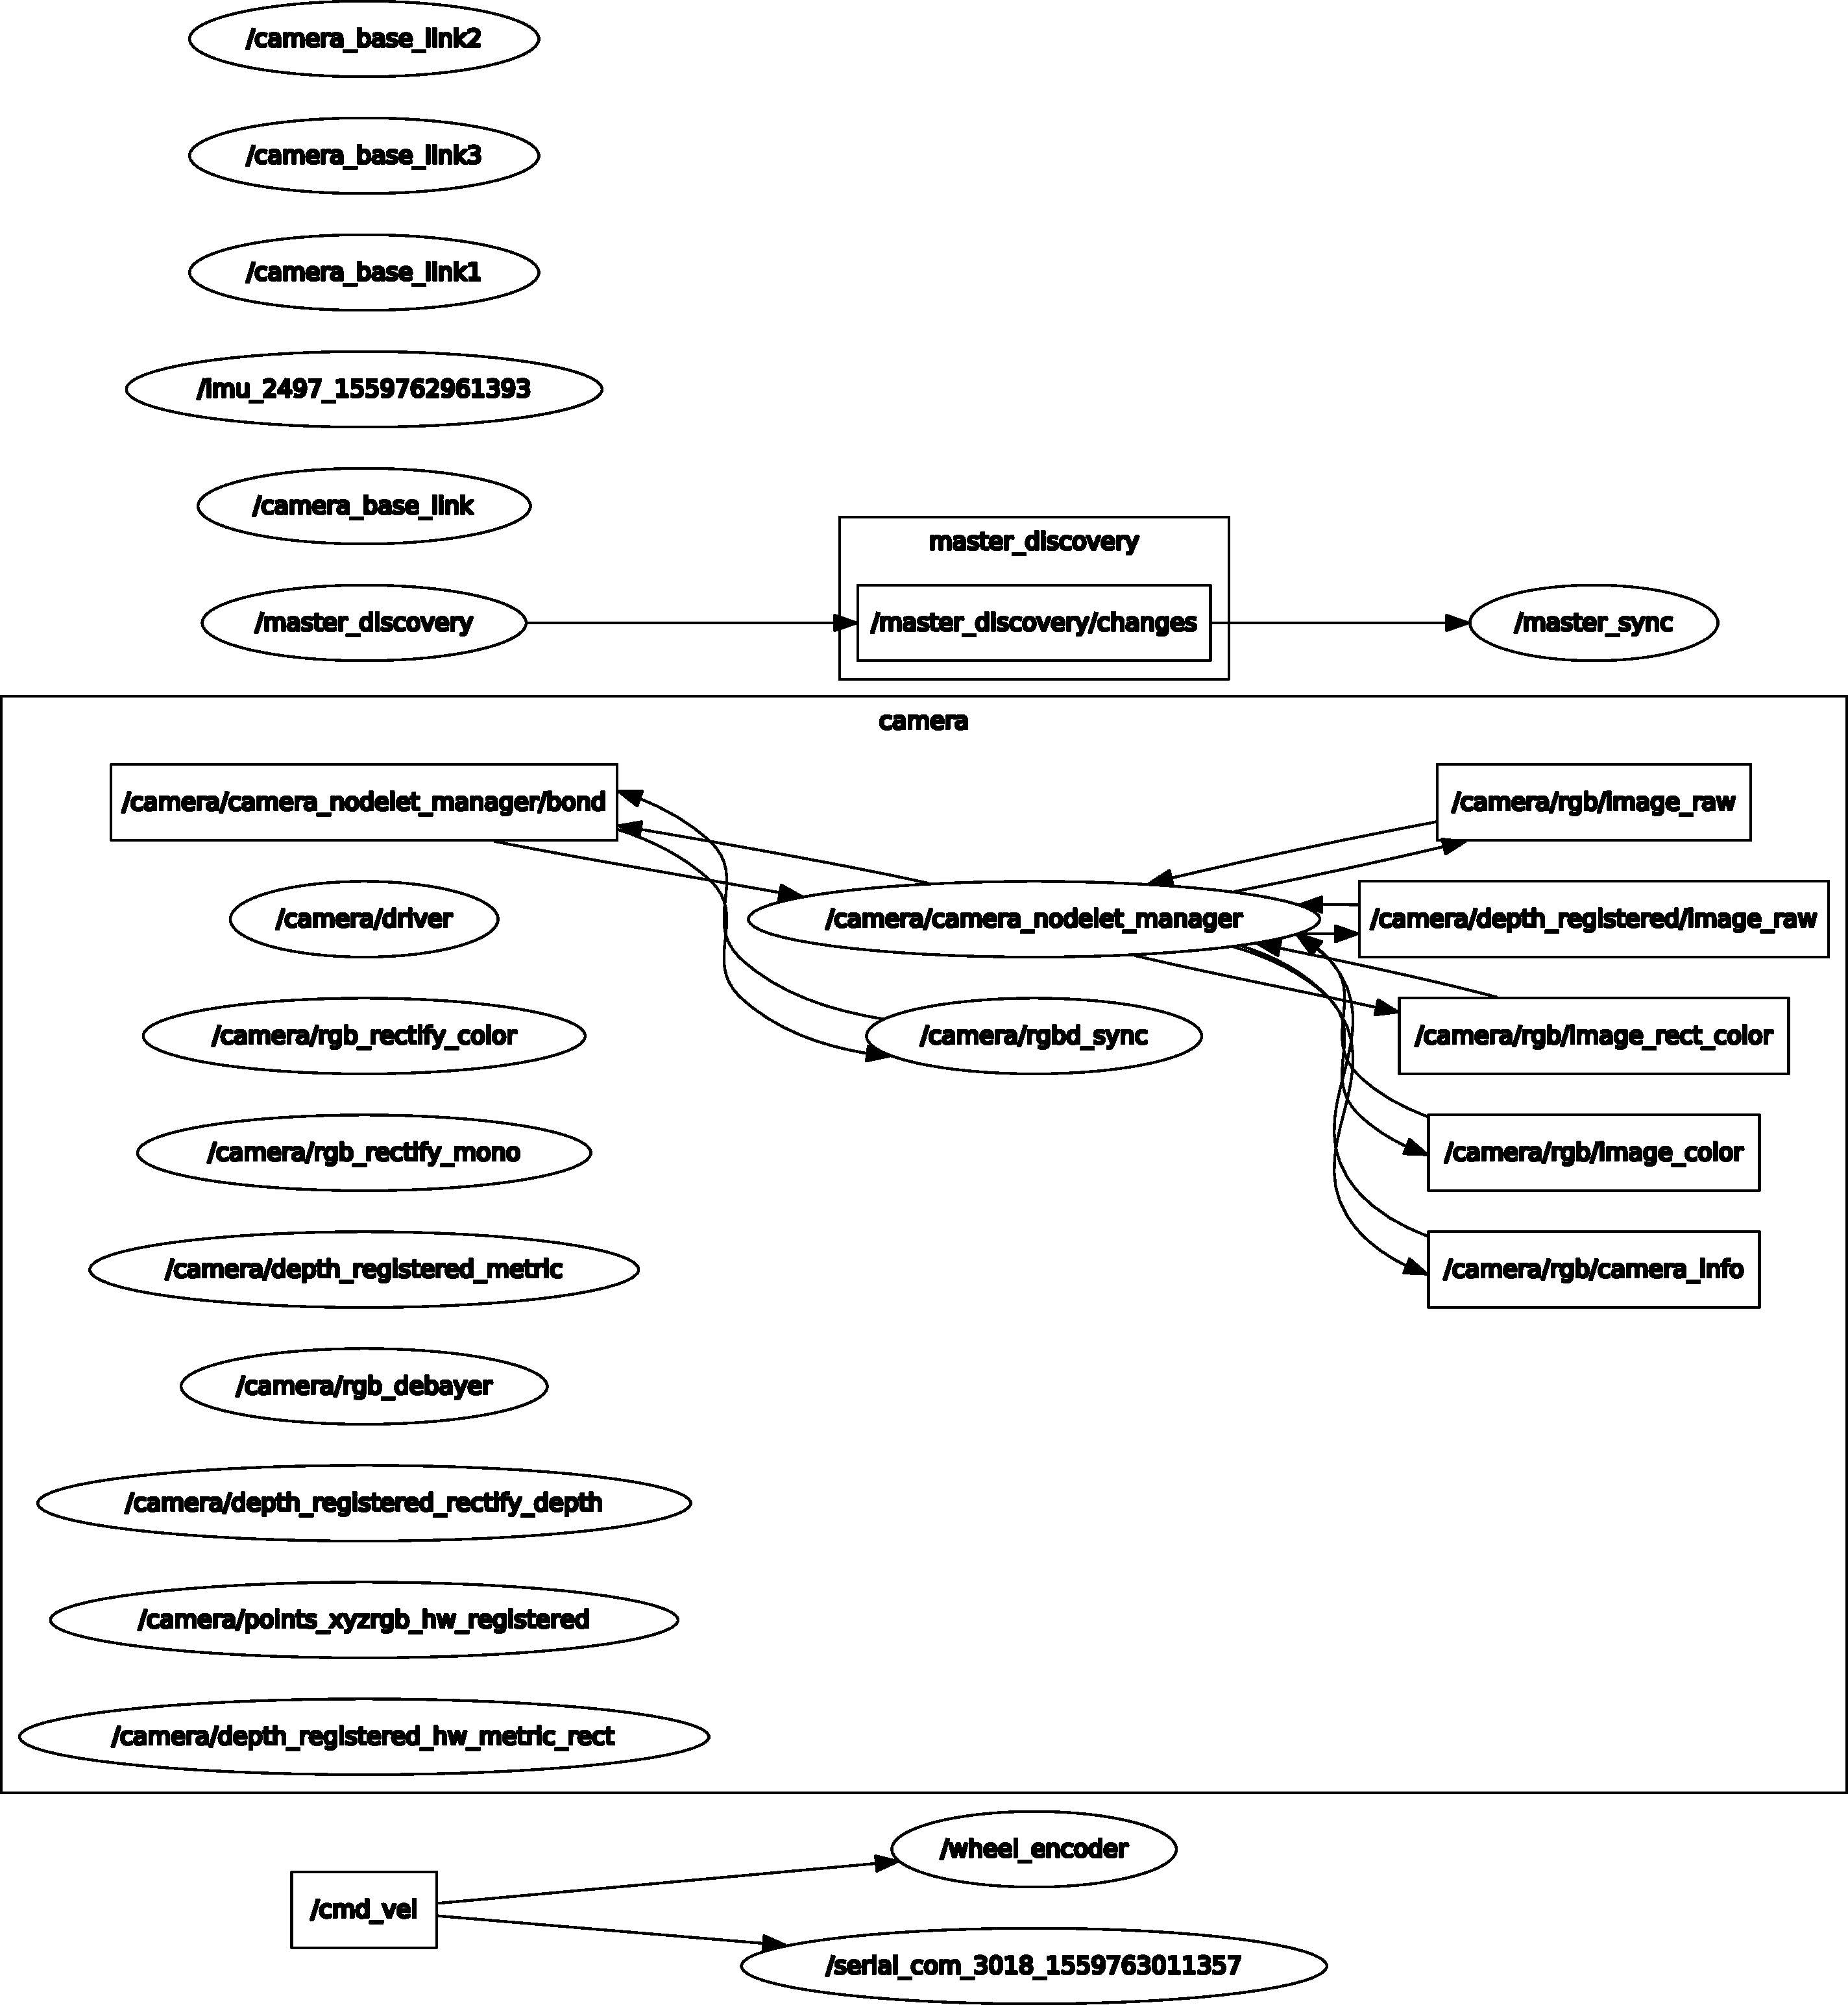
\includegraphics[width=.8\textwidth]{images/rqt_graphs/rpi_onboardBAG.pdf}
    \caption{Captura de los nodos corriendo dentro de la Rapberry Pi 3B+}
    \label{rqt01}
\end{figure}

\newpage
Si se corriese el SLAM en tiempo real, la arquitectura de nodos de ROS sería la siguiente:

\begin{figure}[!ht]
    \centering
    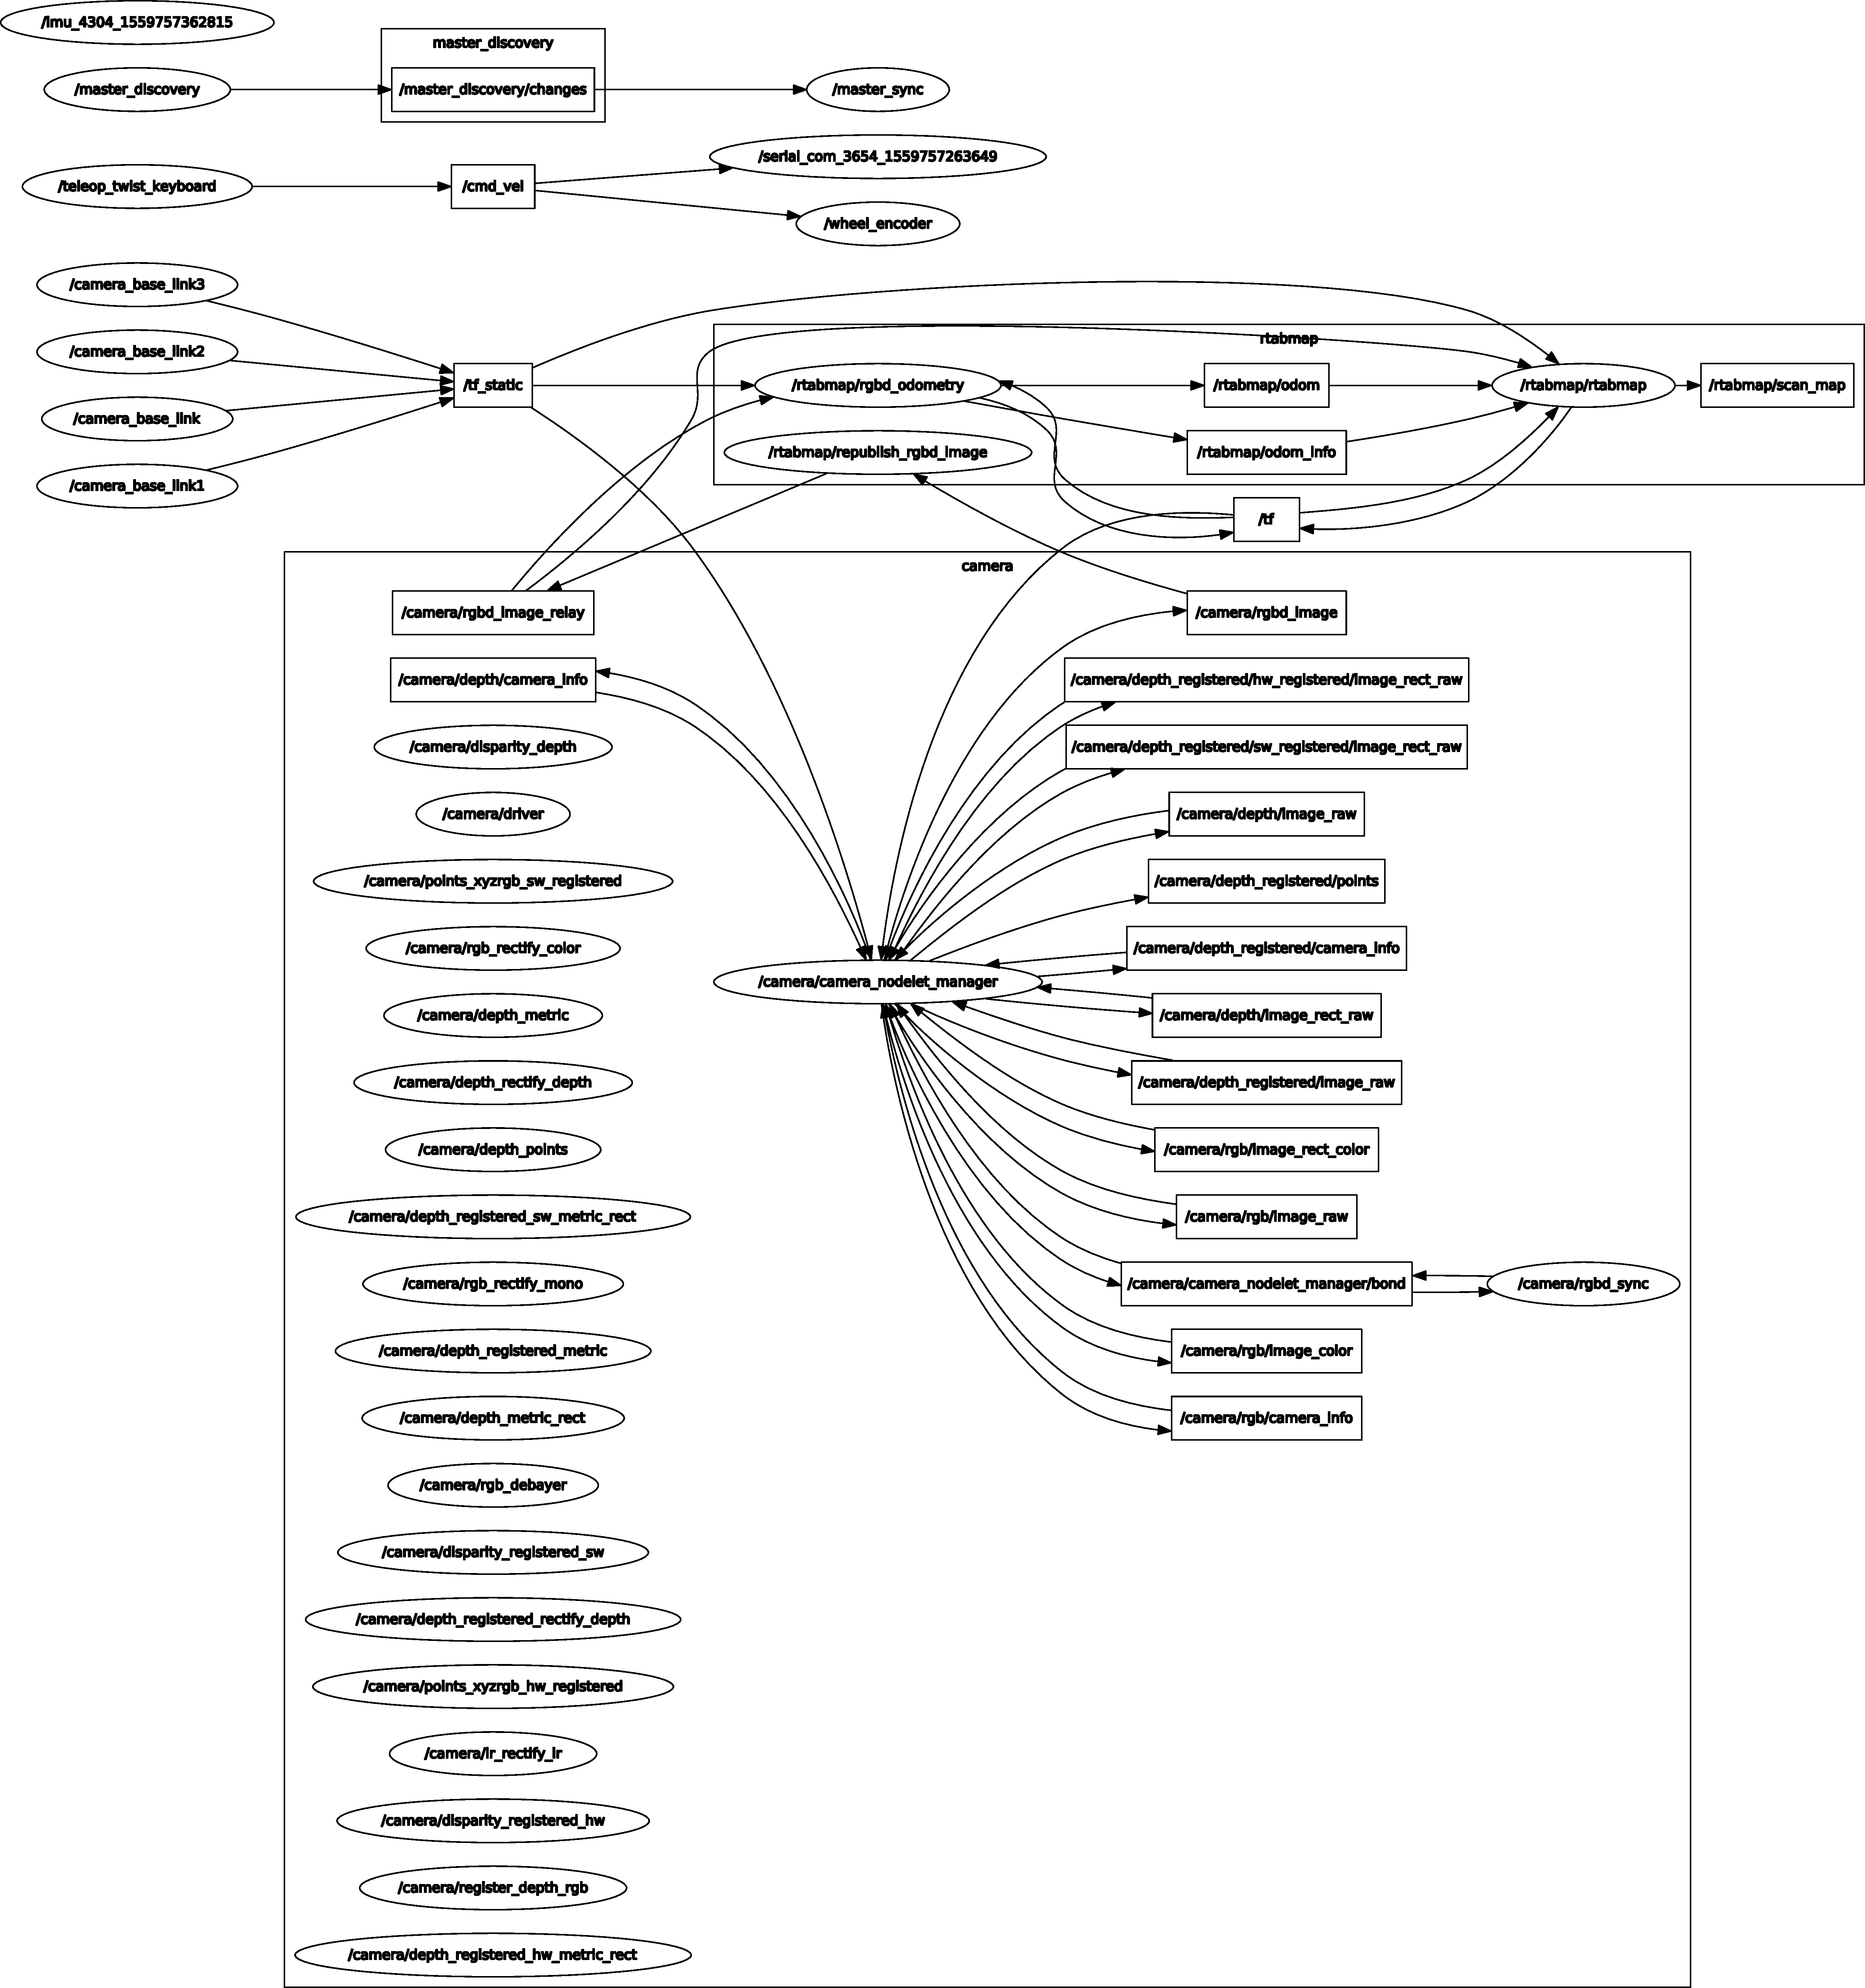
\includegraphics[width=.8\textwidth]{images/rqt_graphs/rpi_onboardSLAM.pdf}
    \caption{Captura de los nodos cuando se realiza SLAM en tiempo real}
    \label{rqt02}
\end{figure}

Para los experimentos, y en concreto con RTAB-Map, la estructura nodal es la siguiente:
\begin{figure}[!ht]
    \centering
    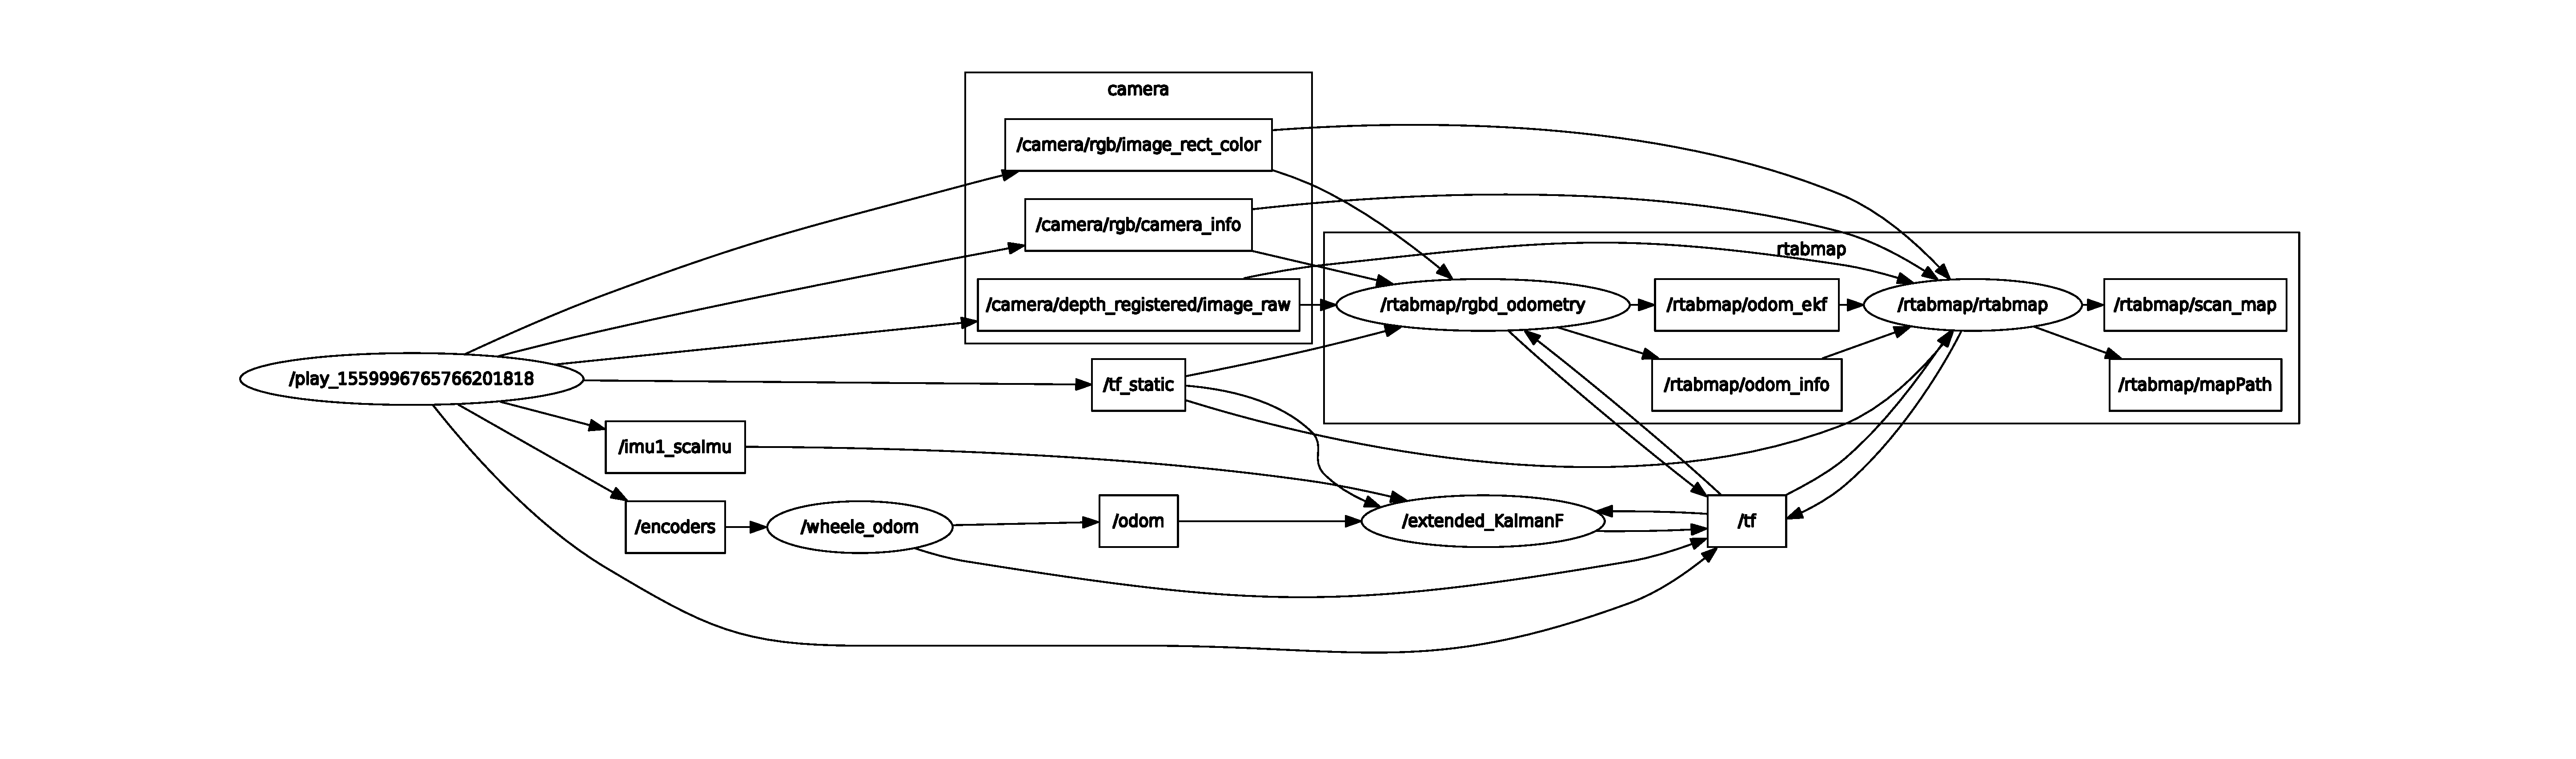
\includegraphics[width=.8\textwidth]{images/rqt_graphs/graph_RTABMAP.pdf}
    \caption{Captura de los nodos ejecutandose cuando se corre SLAM sobre los bags}
    \label{rqt03}
\end{figure}

\section{Puntos destacables de la implementación del proyecto}

\subsection{Obtención de los parámetros de la cámara}
Destacar que, siempre es necesario conocer los parámetros intrínsecos de la cámara además de la matriz de rotación. Para obtener la matriz de parámetros de nuestra cámara, se ha hecho uso del paquete de ROS, \textit{\href{http://wiki.ros.org/camera_calibration}{Camera\_calibration}}.\\
Este paquete nos proporcionará la herramienta mostrada a continuación, que gracias a un tablero de ajedrez nos dará los parámetros intrínsecos de nuestra cámara:
\begin{figure}[!ht]
    \centering
    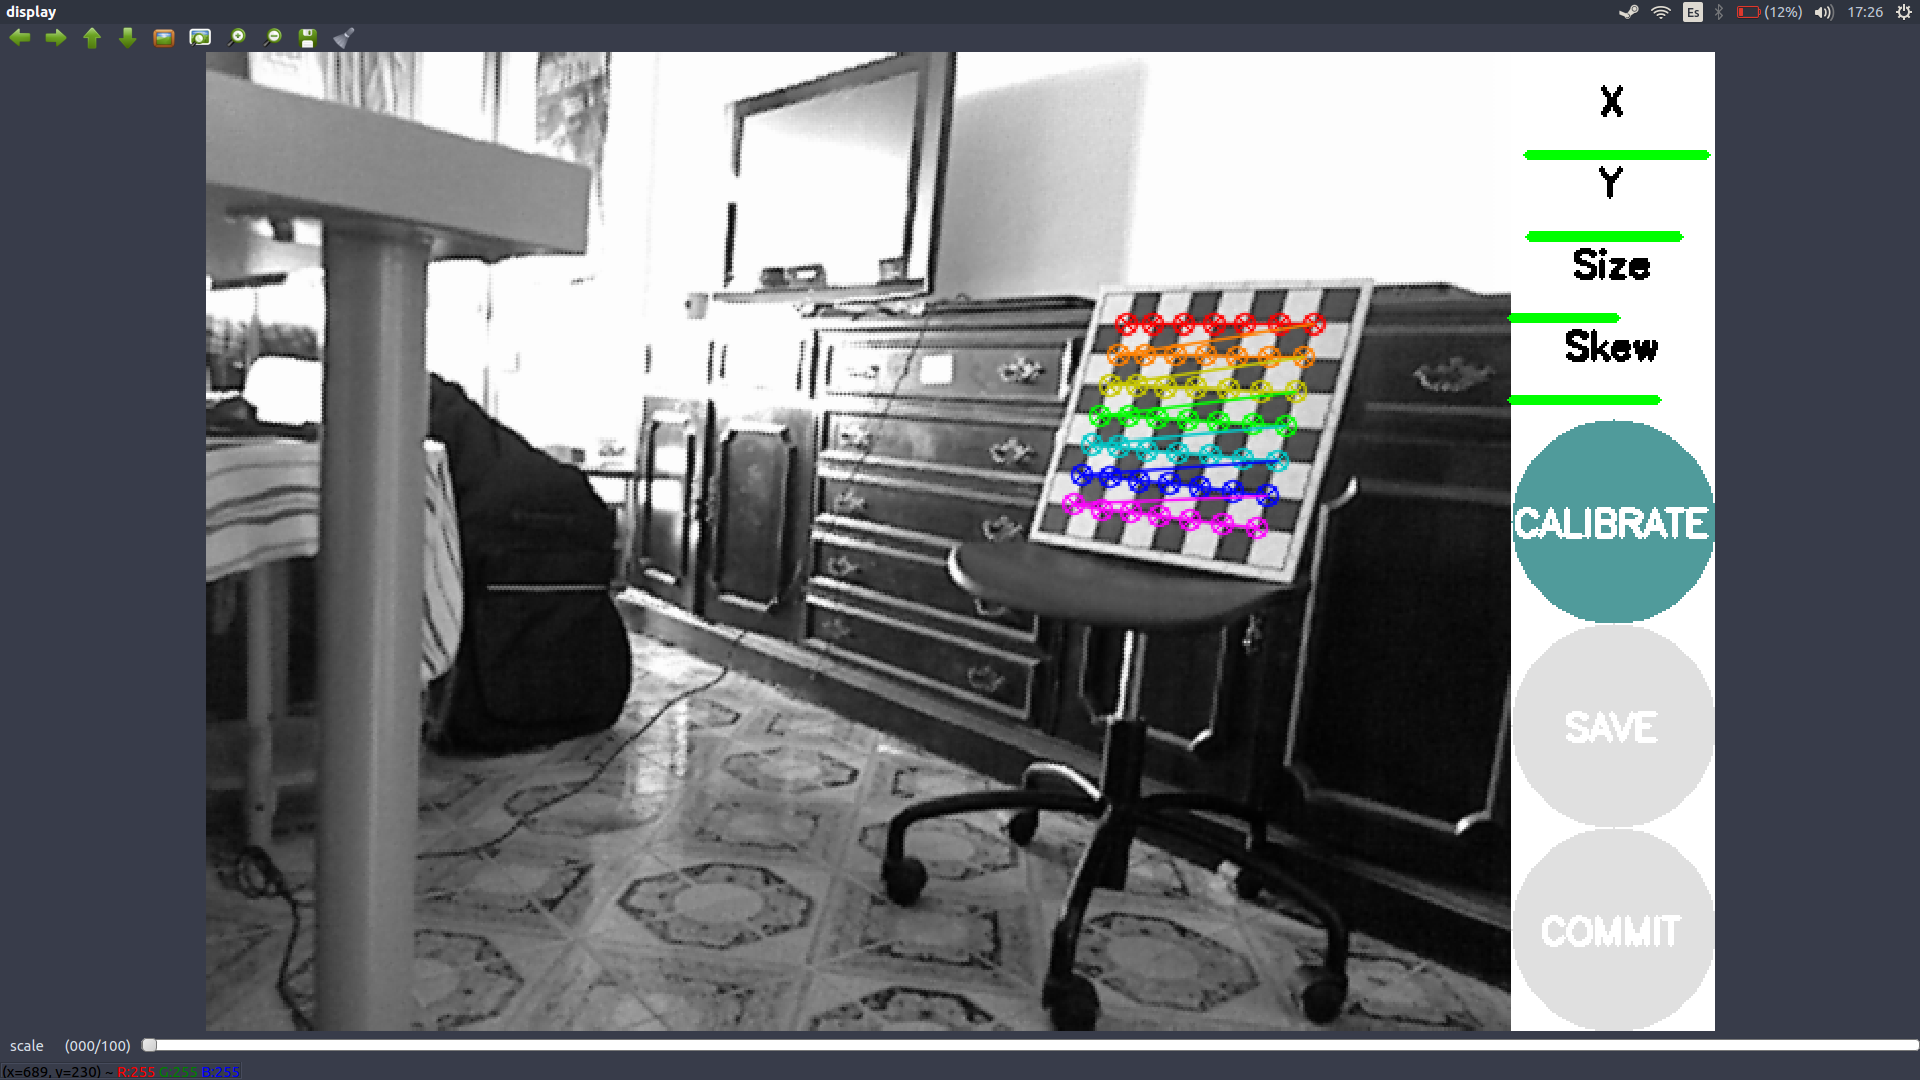
\includegraphics[width=0.57\textwidth]{images/calibration_art}
    \caption{GUI proporcionada por el paquete ejecutándose}
\end{figure}

Las matrices serán dadas en pormato \textit{.ost} y \textit{.yaml} que, despues se le pasará cuando se quiera emplear la cámara para actualizar el topic camera\_info,cuyo 
tipo de mensaje será \textit{\href{http://docs.ros.org/melodic/api/sensor_msgs/html/msg/CameraInfo.html}{sensor\_msgs/CameraInfo}}.
\subsection{Inicialización del robot}
Para lanzar todos los nodos de ROS en el ordenador de abordo del robot y en el ordenador principal se han creado los siguientes ficheros \textit{roslaunch}:
    \begin{figure}[!ht]
        \centering
        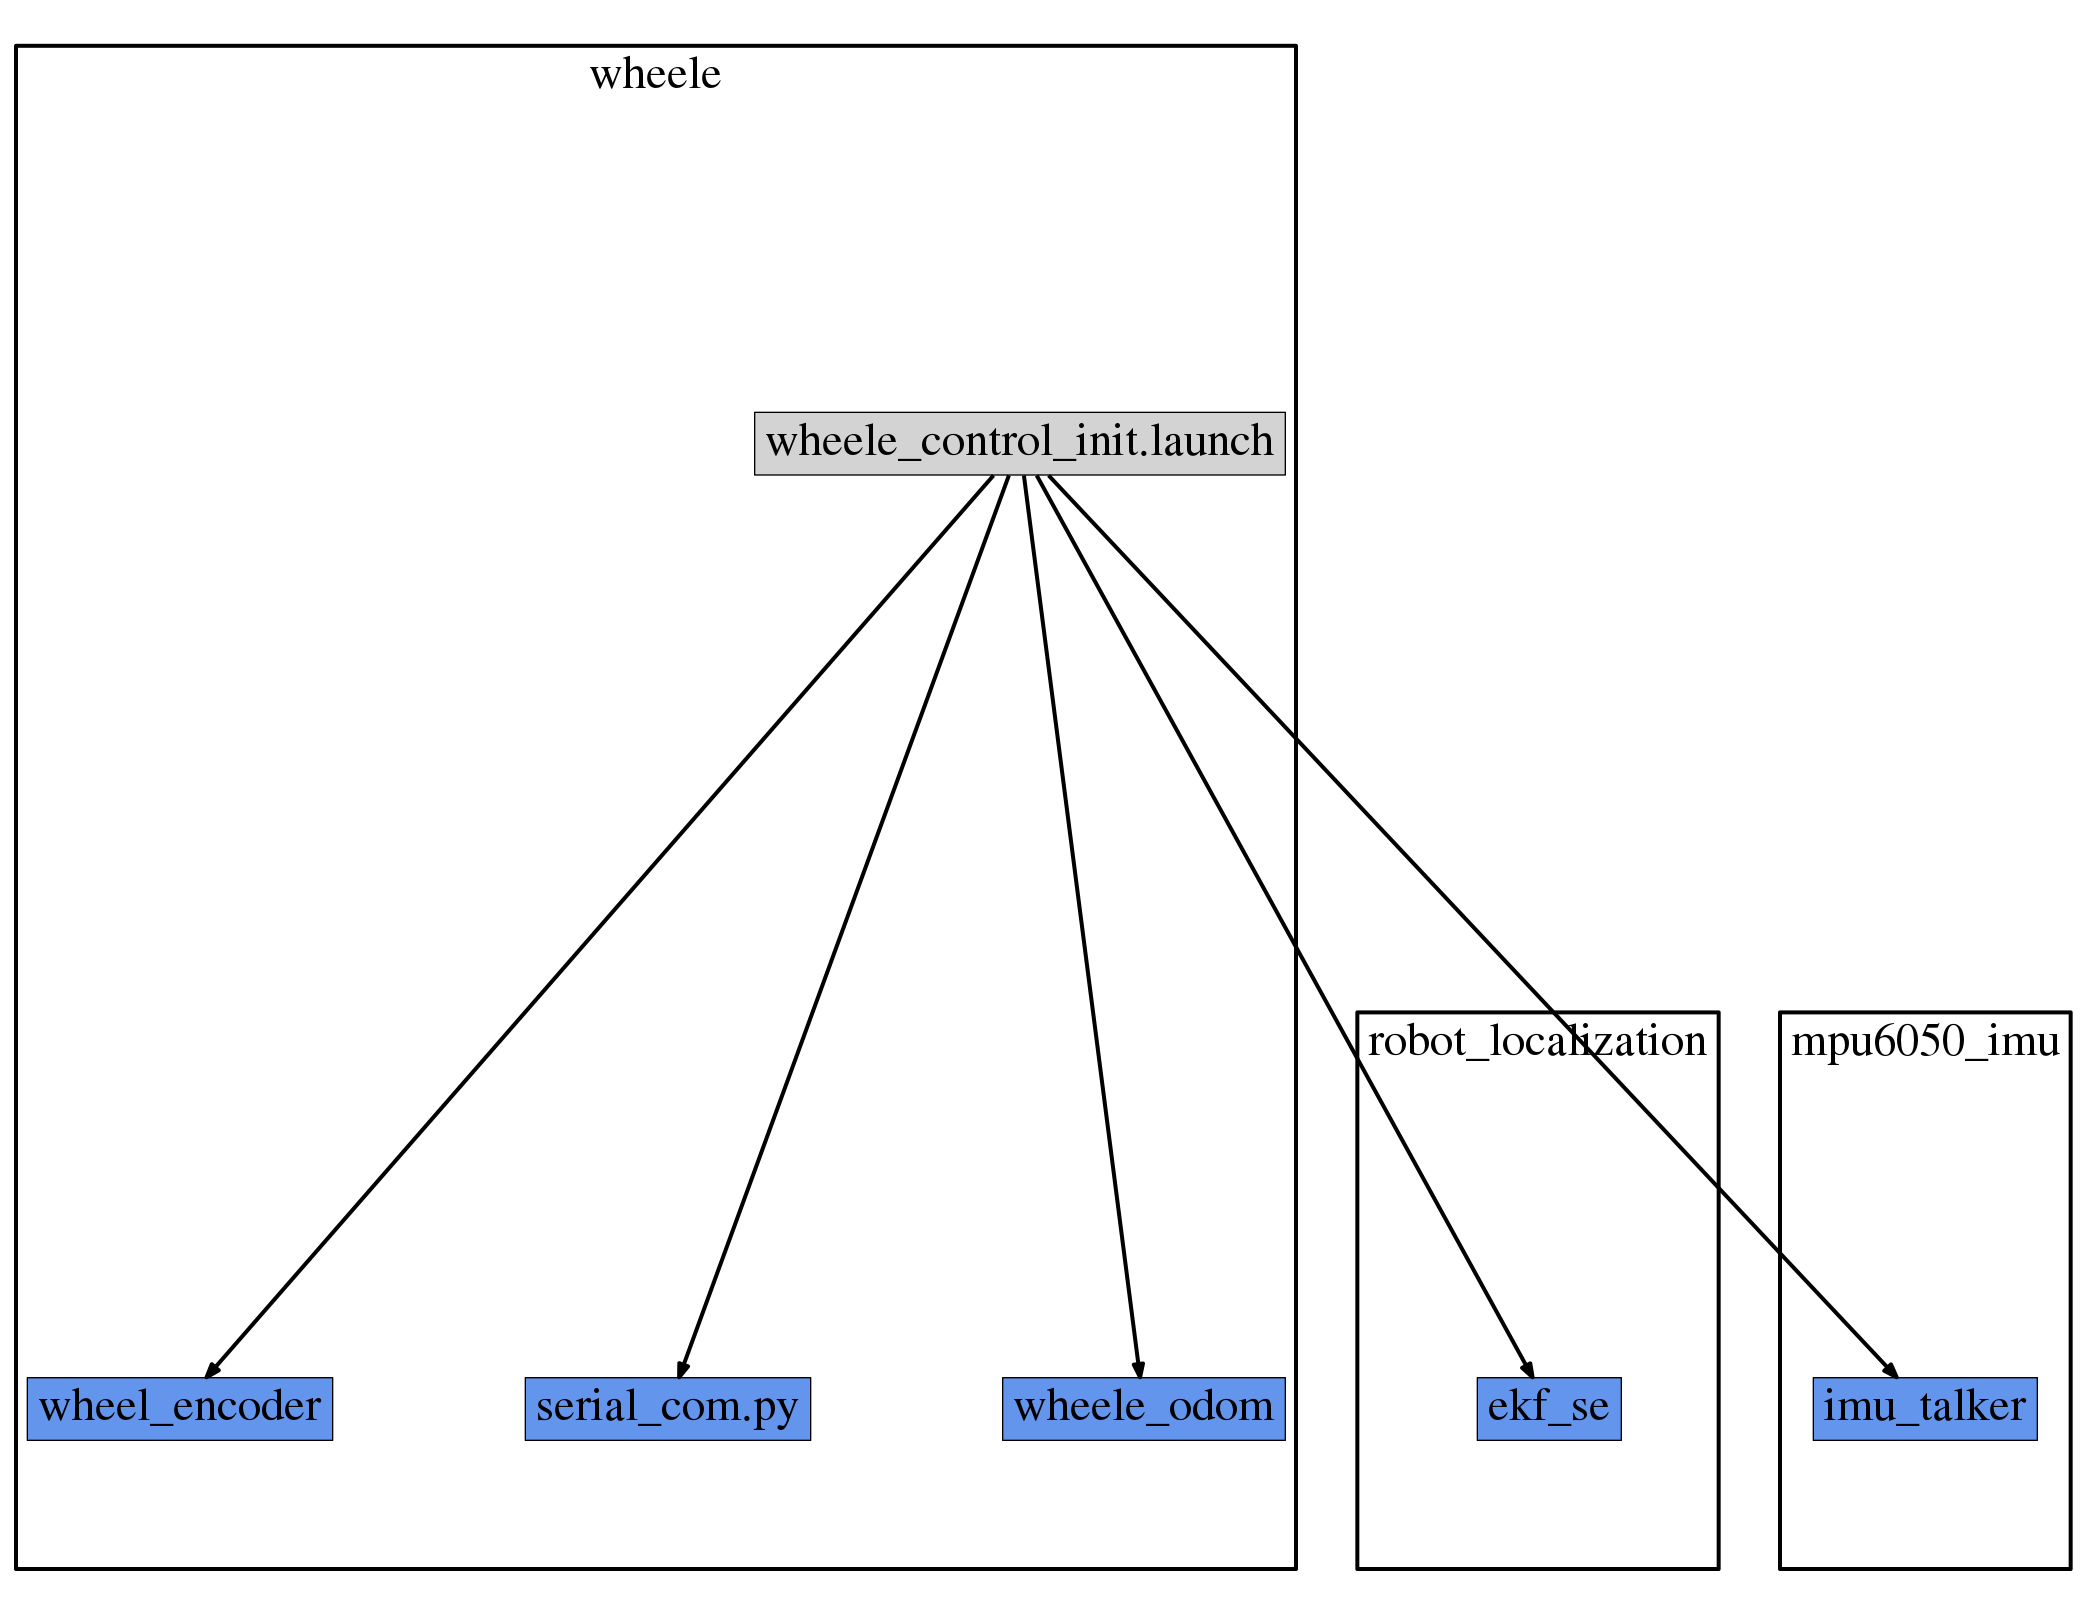
\includegraphics[width=0.57\textwidth]{images/whee}
        \caption{Nodos lanzados en el robot}
    \end{figure}

También se lanzarán los drivers de la cámara, aunque no aparezcan en la imagen. Los drivers son proporcionados por el 
paquete de ROS \textit{\href{https://github.com/ros-drivers/freenect\_stack}{Freenect}}.
Para poder tener control del motor integrado en la cámara, se ha empleado el paquete \textit{\href{https://github.com/muhrix/kinect_aux}{Kinect-aux}}.
    


